\section{Result}
\label{Result}
Based on the experimental results that have been applied the application of the method has been successfully applied.
From the experimental results obtained:
\begin{enumerate}
    \item 
    if the card has not been registered then the card can not be read by system and will notification "Card is not Register".
    \item
    If the inserted OTP code does not match the code sent to the feeding user's account it will be rejected by the system and on the LCD it will display the notification of 'Invalid OTP Code'.
    \item
    If the OTP code and the card is in accordance then the data will be stored and the LCD will show the notification 'Thank you'
    \item
    The system can only be accessed using a predefined IP that is 192.168.1.102
    \item
    OTP code will be different every day and will be automatically generated when user tapping.
\end{enumerate}

Here are the results of the OTP code that was successfully sent to the user's account or card owner.
\begin{figure}[ht]
\begin{center}
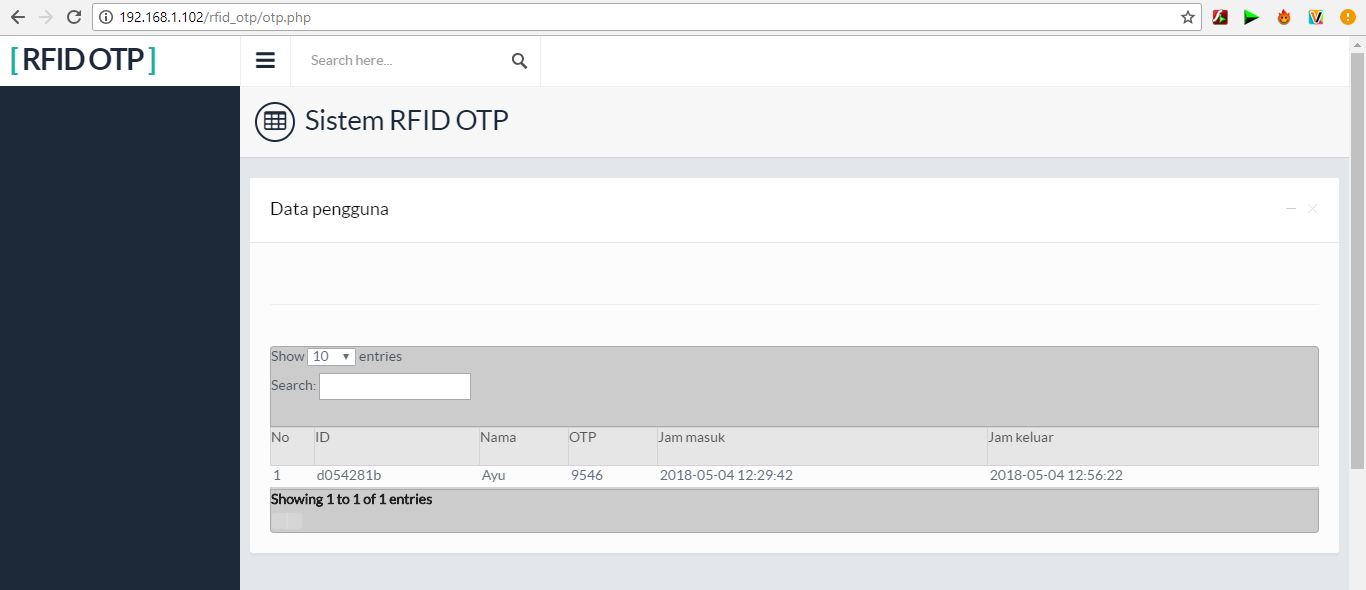
\includegraphics[width=12cm]{figures/OTP1.JPG}
\end{center}
\caption{User Account.
\label{eq:30}}
\end{figure}  

\begin{figure}[ht]
\begin{center}
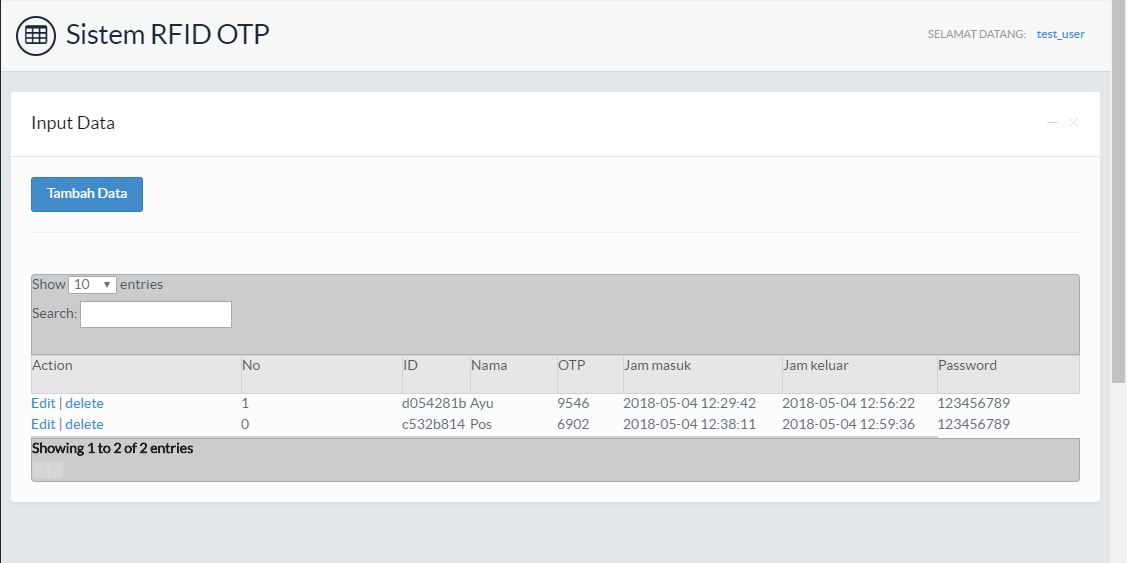
\includegraphics[width=12cm]{figures/AdminOTP.JPG}
\end{center}
\caption{Admin.
\label{eq:30}}
\end{figure}  


